\documentclass{standalone}
\usepackage{tikz}
\usepackage{ctex,siunitx}
\setCJKmainfont{Noto Serif CJK SC}
\usepackage{tkz-euclide}
\usepackage{amsmath}
\usepackage{wasysym}
\usetikzlibrary{patterns, calc}
\usetikzlibrary {decorations.pathmorphing, decorations.pathreplacing, decorations.shapes,}
\begin{document}
\small
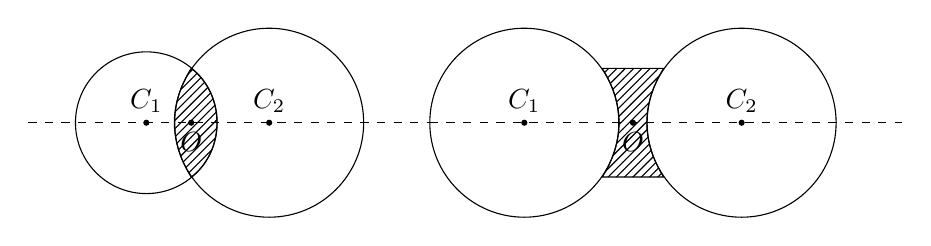
\begin{tikzpicture}[>=latex,scale=0.6]
  \draw [dashed](-3.5,0)--(5,0);
  \draw (-1,0) circle (1.5);
  \draw (1.6,0) circle(2);
  \node at (-1,0)[above]{$C_1$};
  \node at (1.6,0)[above]{$C_2$};
  \node at (-0.05,0)[below]{$O$};
  \draw [fill=black] (-1,0) circle (1.5pt);
  \draw [fill=black] (1.6,0) circle (1.5pt);
  \draw [fill=black] (-0.05,0) circle (1.5pt);
  \draw [pattern=north east lines](-0.05,1.15) to [bend right=32] (-0.05,-1.15) to [bend right=54](-0.05,1.15);
  \begin{scope}[xshift=8cm]
    \draw [dashed](-3,0)--(7,0);
    \draw (-1,0) circle (2);
    \draw (3.6,0) circle(2);
    \node at (-1,0)[above]{$C_1$};
    \node at (3.6,0)[above]{$C_2$};
    \node at (1.3,0)[below]{$O$};
    \draw [fill=black] (-1,0) circle (1.5pt);
    \draw [fill=black] (3.6,0) circle (1.5pt);
    \draw [fill=black] (1.3,0) circle (1.5pt);
    \draw [pattern=north east lines](.65,1.15) to [bend left=32] (.65,-1.15) --(1.95,-1.15) to [bend left=32](1.95,1.15)--(.65,1.15);
  \end{scope}
\end{tikzpicture}
\end{document}